\documentclass[conference]{IEEEtran}

\usepackage{cite}
\usepackage{amsmath,amssymb,amsfonts}
\usepackage{graphicx}
\usepackage{textcomp}
\usepackage{xcolor}
\usepackage{booktabs}
\usepackage{hyperref}
\usepackage{balance}

\hypersetup{
    colorlinks=true,
    linkcolor=black,
    citecolor=black,
    urlcolor=blue
}

\def\BibTeX{{\rm B\kern-.05em{\sc i\kern-.025em b}\kern-.08em
    T\kern-.1667em\lower.7ex\hbox{E}\kern-.125emX}}

% IEEE conference papers carry no page numbers.
\pagestyle{empty}

\begin{document}

\title{How Much of Fake Review Detection on YelpCHI is Business Memorization?}

\author{
\IEEEauthorblockN{Rohan Mukka}
\IEEEauthorblockA{\textit{School of Computer Science}\\
\textit{University of Oklahoma}\\
Norman, OK, USA\\
rohan.mukka-1@ou.edu}
\and
\IEEEauthorblockN{Rithwik Reddy Donthi Reddy}
\IEEEauthorblockA{\textit{School of Computer Science}\\
\textit{University of Oklahoma}\\
Norman, OK, USA\\
rithwikreddyd@ou.edu}
}

\maketitle

% ============================================================
% ABSTRACT
% ============================================================

\begin{abstract}
YelpCHI is the standard benchmark for fake review detection, and reported
accuracies on it are high. We show that much of that performance does not come
from detecting deception. Fake reviews in YelpCHI are concentrated by business:
657 of its 1{,}224 businesses contain no fake reviews at all, and the
per-business fake rate is by itself a 0.951-AUC predictor of the label. Any
split that lets a business appear in both training and test folds therefore
partly measures memorization of which businesses were spam targets. We build
ReviewGuard, a detector fusing a lexical text representation with reviewer- and
business-level behavioral features, and evaluate it under two protocols
differing only in how folds are partitioned. Under a reviewer-disjoint split ---
the convention in this literature --- a behavioral random forest reaches 0.934
AUC-ROC; under a business-disjoint split, with identical features, models, and
tuning, it falls to 0.646. Each model's drop tracks its access to business
identity, from 0.032 for a text-only model to 0.289 for the random forest,
which is enough to invert the ranking of behavioral and textual features. We
additionally document two integrity failures in a widely circulated
distribution of the dataset: label-contaminated timestamps yielding 0.965 AUC
from the timestamp alone, and a behavioral feature file uncorrelated with both
the label and its own column definitions. We argue that business-disjoint
evaluation should be reported alongside any YelpCHI result.
\end{abstract}

\begin{IEEEkeywords}
fake review detection, evaluation methodology, data leakage, YelpCHI,
reviewer behavior, focal loss, multi-modal fusion
\end{IEEEkeywords}

% ============================================================
% I. INTRODUCTION
% ============================================================

\section{Introduction}

Online review platforms are consequential enough that manipulating them is
profitable. Luca and Zervas estimate that review fraud is economically
significant at the scale of entire markets~\cite{luca2016fake}, and the
availability of fluent text generation has lowered the cost of producing
plausible fake content~\cite{crothers2023machine}. A large research literature
has responded with detectors that combine review text with reviewer behavior,
and reported numbers on the standard benchmark --- YelpCHI~\cite{rayana2015collective}
--- are strong.

This paper began as an attempt to build such a detector. In the course of doing
so we found that the benchmark rewards a shortcut that has little to do with
deception, and that the headline numbers a straightforward pipeline produces are
largely an artifact of how the data is partitioned.

The mechanism is simple. YelpCHI was assembled by collecting reviews for a set
of Chicago businesses. Spam campaigns target particular businesses, so the label
is concentrated by business rather than spread uniformly: 657 of the 1{,}224
businesses in the corpus contain zero fake reviews, the median business has a
fake rate of exactly zero, and mapping each review to the fake rate of its
business yields an AUC of 0.951 on its own. A model given any feature that
identifies the business --- its review count, its rating distribution, or a
rating deviation computed against its mean --- can score well by learning which
businesses are spam targets, and will not transfer to a business it has not
seen.

We therefore evaluate under two protocols that are identical except for the
grouping variable used to form cross-validation folds. The
\textit{reviewer-disjoint} protocol guarantees that no reviewer spans the split,
which is the precaution the literature normally takes. The
\textit{business-disjoint} protocol additionally guarantees that no business
spans the split, so a model must generalize to businesses it has never
observed. The gap between them measures the shortcut.

Our contributions are:

\begin{enumerate}
\item A quantification of business-identity leakage in YelpCHI
      (Section~\ref{sec:integrity}), and a demonstration that it accounts for
      the majority of the apparent performance of behavioral fake review
      detectors on this benchmark (Section~\ref{sec:results}).
\item ReviewGuard, a two-branch detector fusing lexical text features with
      reviewer and business behavioral features, trained with focal loss under
      severe class imbalance, evaluated under both protocols with per-model
      threshold tuning so that baselines are not handicapped
      (Section~\ref{sec:method}).
\item A data integrity audit of a widely circulated CSV distribution of
      YelpCHI, identifying label-contaminated timestamps and an uninformative
      behavioral feature file, both excluded from our experiments
      (Section~\ref{sec:integrity}).
\item Evidence that the fusion benefit, unlike the behavioral advantage,
      survives the stricter protocol --- alongside the observation that all
      absolute performance under it is far below what this benchmark is
      usually reported to support (Section~\ref{sec:results}).
\end{enumerate}

% ============================================================
% II. RELATED WORK
% ============================================================

\section{Related Work}
\label{sec:related}

\subsection{Detection Methods}

Early work treated deceptive review detection as text classification. Ott et
al.~\cite{ott2011finding} showed that $n$-gram and psycholinguistic features
separate solicited deceptive reviews from genuine ones with near-human accuracy
in a controlled corpus. Jindal and Liu~\cite{jindal2008opinion} introduced
opinion spam as a distinct problem and applied duplicate detection and
engineered features at scale. Mukherjee et al.~\cite{mukherjee2013what} made the
central observation that motivates two-branch designs: reviewer behavior ---
posting bursts, rating extremity, activity patterns --- carries signal that text
alone does not, and combining the two beats either.

Representation learning followed. Recurrent and convolutional models replaced
hand-built lexical features, and pre-trained transformers~\cite{devlin2019bert,
liu2019roberta} became the default text encoder, consistently improving on
bag-of-words baselines for review classification. Most recently the review
ecosystem has been modeled as a heterogeneous graph over reviewers, businesses,
and reviews. Rayana and Akoglu~\cite{rayana2015collective} propagate spam
evidence through reviewer--product networks, and graph neural
networks~\cite{kipf2017semi, wang2020attributed} learn representations over the
same structure. The YelpCHI distribution used by much of this line of work
descends from Rayana and Akoglu's release.

\subsection{Evaluation and Leakage}

Our concern is orthogonal to the choice of model. Kaufman et
al.~\cite{kaufman2012leakage} characterize leakage as the introduction of
information about the target that would be unavailable at prediction time, and
document how easily it survives into published results. Benchmark-specific
shortcut learning is now well documented across machine
learning~\cite{geirhos2020shortcut}: models reach high accuracy through features
that correlate with the label in the dataset's construction rather than in the
phenomenon.

Graph-based fake review detectors are structurally exposed to the effect we
describe, because the reviewer--business graph makes business identity directly
available. This does not invalidate that work --- in a deployment where a
platform monitors a fixed, known set of businesses, exploiting business-level
priors is legitimate. The problem is that the standard random or
reviewer-grouped split does not distinguish between a detector that generalizes
to new businesses and one that has learned a lookup table of past spam targets,
and results are usually not reported in a way that separates the two.

% ============================================================
% III. DATA INTEGRITY AUDIT
% ============================================================

\section{Data Integrity Audit}
\label{sec:integrity}

We work from a CSV distribution of YelpCHI containing 45{,}954 reviews with
review text, reviewer and business identifiers, star ratings, timestamps, and
labels; 6{,}677 reviews (14.53\%) are labeled fake. The review counts, label
counts, and class balance match the canonical \texttt{.mat} release. Before
using any column we audited it. Two sources failed, and are excluded from every
experiment in this paper. Table~\ref{tab:integrity} summarizes the diagnostics.

% generated by src/make_tables.py -- do not edit
\begin{table}[htbp]
\caption{Data integrity audit. The first two blocks describe inputs excluded
from the study; the third describes a property of YelpCHI itself that dictates
the evaluation protocol.}
\label{tab:integrity}
\centering
\footnotesize
\setlength{\tabcolsep}{4pt}
\begin{tabular}{@{}llr@{}}
\toprule
\textbf{Source} & \textbf{Diagnostic} & \textbf{Value} \\
\midrule
\texttt{date} column & AUC from timestamp alone & 0.965 \\
 & Monthly fake-rate range & 0.026--0.498 \\
 & Distinct seconds values & 1 \\
\texttt{behavioral\_} & Max $|r|$ vs.\ own definition & 0.005 \\
\texttt{features.csv} & Max $|r|$ vs.\ label & 0.008 \\
Business identity & Businesses with no fakes & 657/1224 \\
 & AUC from business fake rate & 0.951 \\
\bottomrule
\end{tabular}
\end{table}


\subsection{Contaminated Timestamps}

The released \texttt{date} column does not behave like a record of when reviews
were posted. A random forest given nothing but the raw Unix timestamp separates
fake from genuine reviews with an AUC of 0.965. The monthly fake rate swings
from 49.8\% in January 2010 to 2.6\% in March 2010, and the entire corpus spans
111 days, against the multi-year range of the original Yelp collection.
Meanwhile the within-day structure is absent: posting hours are uniform across
all 24 hours to within a factor of 1.11, and the seconds field takes exactly one
distinct value.

The combination is diagnostic. Real posting times are strongly diurnal, so a
uniform hour distribution and a constant seconds field indicate that the time
component was generated rather than observed; and a label association this
strong within a four-month window indicates that whatever generated the dates
was conditioned on the class. Every temporal behavioral feature in the standard
repertoire --- posting burstiness, inter-review gaps, account age at review ---
would be computed from this column and would inherit the contamination. We
therefore exclude timestamps entirely. This costs us the burstiness features
that Mukherjee et al.~\cite{mukherjee2013what} found informative, and we note it
as a limitation rather than a design choice.

\subsection{An Uninformative Feature File}

The same distribution ships a six-column feature file,
\texttt{behavioral\_features.csv}, holding average star rating, review count,
burst ratio, rating deviation, category diversity, and account age.
Reconstructing each column from the review table it purports to summarize ---
for instance, computing each reviewer's actual mean rating --- yields
correlations of at most 0.005 with the shipped values. The columns also correlate with the label at most 0.008 in
absolute value, and are near-degenerate: the burst ratio is zero for 97.5\% of
rows and category diversity is 1.0 for 99.4\%. The file carries no recoverable
information and we do not use it. We flag it because it is distributed alongside
otherwise usable data and its filename invites use without inspection.

\subsection{Business-Concentrated Labels}

The third finding is a property of YelpCHI itself rather than a defect in a
redistribution, and it is the one that shapes our evaluation. Fake reviews are
concentrated by business: 657 of 1{,}224 businesses contain no fake reviews, 58
consist entirely of fake reviews, and the median business fake rate is zero.
Mapping each review to its business's fake rate gives an AUC of 0.951.
Fig.~\ref{fig:concentration} shows the distribution.

\begin{figure*}[t]
\centering
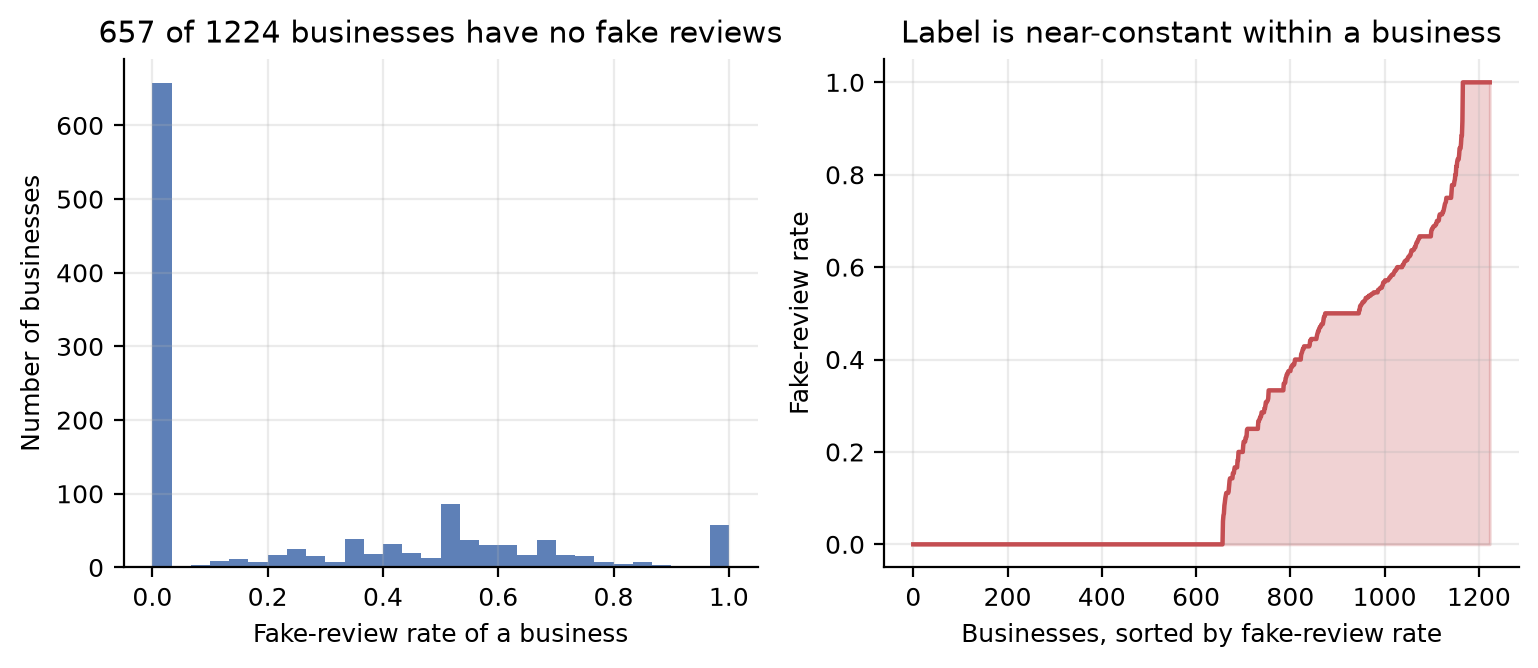
\includegraphics[width=0.88\textwidth]{figures/business_label_concentration.png}
\caption{Fake reviews are concentrated by business. Left: distribution of
per-business fake rates; the mode at zero is 657 businesses with no fake reviews
at all. Right: businesses sorted by fake rate, showing that the label is
near-constant within a business.}
\label{fig:concentration}
\end{figure*}

This is not an error --- it reflects how spam campaigns actually work, and how
the corpus was collected. But it means that business identity is close to a
sufficient statistic for the label, and that any feature which encodes business
identity is a shortcut.

% ============================================================
% IV. METHOD
% ============================================================

\section{ReviewGuard}
\label{sec:method}

\subsection{Problem Formulation}

Given a review $r = (t, b)$ with text $t$ and behavioral context $b$, we learn
$f : (t, b) \rightarrow [0,1]$ estimating $P(\text{fake} \mid t, b)$. Positives
are reviews labeled as spam in the YelpCHI ground truth.

\subsection{Text Branch}

The text branch encodes the review's actual text. We compute two TF-IDF
representations --- word unigrams and bigrams, and character $n$-grams of length
three to five with word-boundary padding --- each capped at 50{,}000 features
with a minimum document frequency of five and sublinear term frequency scaling.
Character $n$-grams are included because they are robust to the spelling
irregularity and punctuation patterns that distinguish review registers. The two
matrices are concatenated and reduced by truncated SVD to a 256-dimensional
dense vector, which is the representation handed to the fusion model.

To this we append ten stylometric features in the tradition of Ott et
al.~\cite{ott2011finding}: character and word counts, mean word length,
capitalization, exclamation, question mark, digit and punctuation ratios,
first-person pronoun ratio, and type--token ratio. The text branch therefore
contributes 266 dimensions.

\subsection{On the Absence of a Transformer Branch}

The design we set out to evaluate used a fine-tuned RoBERTa-base
encoder~\cite{liu2019roberta} in place of the lexical representation, taking the
768-dimensional \texttt{[CLS]} embedding as the text vector. We report results
with the lexical encoder instead, for an infrastructural reason we state plainly
rather than obscure: the compute environment available for this study had no GPU
and no network route to a pre-trained model repository, so the transformer
branch could not be run. The encoder is implemented and released with our code
so that the comparison can be completed where those resources exist.

This is a real limitation on the text side of our results, and it means our
text branch is a lower bound on what a text branch can do. It does not affect
the paper's central claim, which concerns the evaluation protocol and applies to
any text encoder: the business-disjoint gap we measure is a property of the
benchmark's label structure, not of the representation used.

\subsection{Behavior Branch}

The behavior branch encodes 19 features in three groups. Review-level: star
rating, rating extremity $|{\text{rating}} - 3|$, and review word count.
Reviewer-level: review count, a singleton indicator, mean and standard deviation
of ratings given, ratio of extreme (one- or five-star) ratings, ratio of
positive ratings, number of distinct businesses reviewed, maximum reviews
written for any single business, and mean review length. Business-level: review
count, mean and standard deviation of ratings received, and the signed and
absolute deviation of this review's rating from its business's mean.

Two indicator features, \texttt{rev\_seen\_in\_training} and
\texttt{prod\_seen\_in\_training}, record whether the reviewer and business were
observed during training, making the cold-start case explicit to the model
rather than hiding it in an imputed value.

Crucially, all aggregate tables are fitted on the training rows of a fold and
then applied to held-out rows. A reviewer or business absent from training
receives training-set priors. Computing these aggregates over the full corpus
--- the natural and, in our experience, the default implementation --- leaks
both the existence and the composition of the evaluation fold into the features.

\subsection{Fusion and Training}

The 266-dimensional text vector and the 19-dimensional behavior vector are
standardized and concatenated, then classified by a two-layer MLP: 256 hidden
units, ReLU, dropout 0.3; 64 hidden units, ReLU, dropout 0.3; and a linear
output. Single-branch ablations use the same architecture on one branch alone,
with a smaller $(64, 32)$ hidden configuration for the behavior-only model to
match its input dimensionality.

Training uses focal loss~\cite{lin2017focal},
\begin{equation}
    L = -\alpha_t (1 - p_t)^{\gamma} \log(p_t),
\end{equation}
\noindent with $\gamma = 2$ and $\alpha$ set to the training-set genuine-class
frequency, addressing the 14.53\% positive rate. We optimize with
Adam~\cite{kingma2015adam} at a learning rate of $10^{-3}$, batch size 256, for
at most 40 epochs, retaining the weights with the best validation AUC and
stopping after six epochs without improvement.

% ============================================================
% V. EXPERIMENTAL SETUP
% ============================================================

\section{Experimental Setup}
\label{sec:setup}

\subsection{Two Protocols}
\label{sec:protocol}

Both protocols use five-fold cross-validation, stratified by label, and differ
only in the variable on which folds are made disjoint.

\textbf{Business-disjoint (primary).} Folds are grouped by business identifier,
so every business in a test fold is unseen during training. This is the setting
in which a detector must generalize to businesses it has no history for.

\textbf{Reviewer-disjoint (comparison).} Folds are grouped by reviewer
identifier, so no reviewer spans the split but businesses may. This corresponds
to the precaution commonly taken in this literature.

Within each fold we reserve a grouped, stratified validation slice
(20\% of the training portion, disjoint on the same variable) used for early
stopping and threshold selection. Every fitted object --- TF-IDF vocabularies,
the SVD basis, feature scalers, and the reviewer and business aggregate tables
--- is fit on the fold's training portion alone.

\subsection{Threshold Tuning}

Under 14.53\% positive prevalence, a classifier left at a 0.5 threshold predicts
the majority class almost everywhere, and reporting F1 or recall at that
threshold says more about calibration than about discrimination. We therefore
tune a decision threshold for \textit{every} model, including all baselines, on
the validation slice to maximize Macro-F1, and apply it unchanged to the test
fold. This matters for fair comparison: in a preliminary version of these
experiments, untuned classical baselines recorded fake-class recalls as low as
0.003, which reflects an unadjusted threshold rather than a failure to rank.

\subsection{Baselines}

We compare against four baselines and two ablations: TF-IDF with a linear
SVM~\cite{cortes1995support} and with logistic regression, both on the sparse
lexical matrix; behavioral features with logistic regression and with a random
forest~\cite{breiman2001random}; and the text-only and behavior-only MLPs, which
serve as the fusion ablations.

\subsection{Metrics and Significance}

We report AUC-ROC, average precision, Macro-F1, and fake-class recall, as mean
and standard deviation over the five folds. Average precision is included
because it is the more informative summary under class imbalance. Pairwise
comparisons between ReviewGuard and each baseline use the Wilcoxon signed-rank
test over the five paired fold results. We note the limitation this imposes
explicitly: with $n = 5$ paired observations, the smallest attainable two-sided
$p$-value is 0.0625, so no comparison can reach $\alpha = 0.05$. We report the
$p$-values for completeness and draw conclusions from effect sizes and fold-level
consistency rather than from significance thresholds.

% ============================================================
% VI. RESULTS
% ============================================================

\section{Results}
\label{sec:results}

\subsection{The Protocol Gap}

Table~\ref{tab:protocol} is the paper's central result. It reports AUC-ROC for
every model under both protocols; the models, features, hyperparameters, and
tuning procedure are identical, and only the fold partitioning differs.

% generated by src/make_tables.py -- do not edit
\begin{table}[htbp]
\caption{Effect of the evaluation protocol on AUC-ROC. The reviewer-disjoint
split allows a business to appear in both training and test folds; the
business-disjoint split does not. The gap is the portion of apparent
performance attributable to memorizing which businesses were spam targets.
Rows are ordered by that gap.}
\label{tab:protocol}
\centering
\footnotesize
\setlength{\tabcolsep}{4pt}
\begin{tabular}{@{}lccc@{}}
\toprule
\textbf{Model} & \textbf{Rev.-disj.} & \textbf{Bus.-disj.} & \textbf{Gap} \\
\midrule
Text-only MLP & 0.743 & 0.712 & +0.032 \\
TF-IDF + LogReg & 0.762 & 0.700 & +0.062 \\
TF-IDF + LinearSVM & 0.740 & 0.666 & +0.074 \\
ReviewGuard (Fusion) & 0.856 & 0.730 & +0.126 \\
Behavior-only MLP & 0.889 & 0.706 & +0.183 \\
Behavior + LogReg & 0.782 & 0.599 & +0.183 \\
Behavior + RandomForest & 0.934 & 0.646 & +0.289 \\
\bottomrule
\end{tabular}
\end{table}


\begin{figure*}[t]
\centering
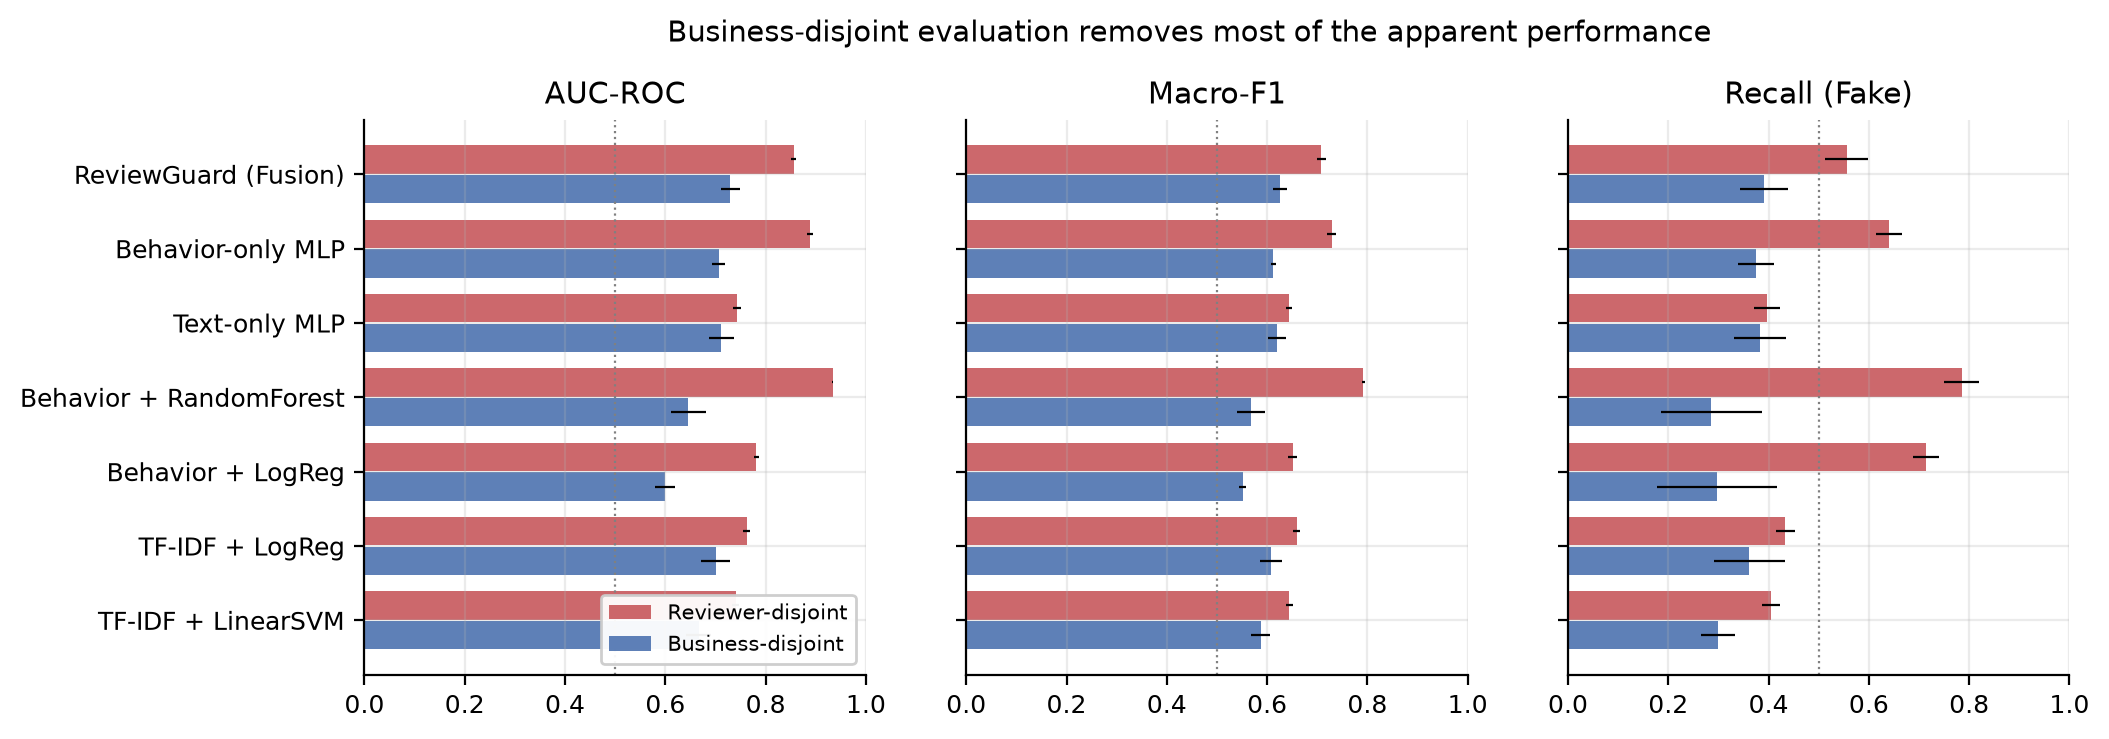
\includegraphics[width=\textwidth]{figures/protocol_comparison.png}
\caption{The same models under both protocols. Bars are means over five folds
with standard deviation whiskers. Behavioral models lose most of their apparent
performance once businesses no longer span the split; text-based models, which
have less access to business identity, lose less.}
\label{fig:protocol}
\end{figure*}

The pattern is consistent, interpretable, and ordered exactly by how much
business identity each model can reach. The text-only MLP loses 0.032 AUC,
because review text identifies its business only weakly. The two TF-IDF
baselines lose 0.062 and 0.074. ReviewGuard, which sees business aggregates
diluted among 266 text dimensions, loses 0.126. The behavior-only models lose
0.183, and the behavioral random forest --- the model best equipped to carve up
a small set of business-level aggregates --- loses 0.289, falling from the best
model in the comparison protocol (0.934) to the worst in the primary one
(0.646).

That reversal is the finding. Under the reviewer-disjoint protocol, the natural
reading of Table~\ref{tab:protocol} is that behavioral features dominate textual
ones for fake review detection on YelpCHI, and that a random forest over 19
behavioral features is the model to beat. Under the business-disjoint protocol
that conclusion inverts. Most of what the behavior branch contributes on this
benchmark is knowing which businesses attract spam, not knowing what a spammer
does.

\subsection{Business-Disjoint Performance}

Table~\ref{tab:results} reports full metrics under the primary protocol.

% generated by src/make_tables.py -- do not edit
\begin{table*}[t]
\caption{Five-fold cross-validated performance on YelpCHI under the
business-disjoint protocol (mean $\pm$ s.d. across folds). Decision thresholds
for every model are tuned on a held-out validation slice to maximise Macro-F1.}
\label{tab:results}
\centering
\small
\begin{tabular}{lcccc}
\toprule
\textbf{Model} & \textbf{AUC-ROC} & \textbf{AP} & \textbf{Macro-F1} & \textbf{Rec(Fake)} \\
\midrule
TF-IDF + LinearSVM & 0.666 $\pm$ 0.024 & 0.265 $\pm$ 0.029 & 0.587 $\pm$ 0.019 & 0.299 $\pm$ 0.034 \\
TF-IDF + LogReg & 0.700 $\pm$ 0.029 & 0.305 $\pm$ 0.038 & 0.608 $\pm$ 0.022 & 0.361 $\pm$ 0.071 \\
Behavior + LogReg & 0.599 $\pm$ 0.020 & 0.201 $\pm$ 0.010 & 0.552 $\pm$ 0.007 & 0.296 $\pm$ 0.120 \\
Behavior + RandomForest & 0.646 $\pm$ 0.035 & 0.221 $\pm$ 0.029 & 0.567 $\pm$ 0.028 & 0.286 $\pm$ 0.101 \\
Text-only MLP & 0.712 $\pm$ 0.025 & 0.325 $\pm$ 0.035 & 0.620 $\pm$ 0.018 & 0.383 $\pm$ 0.051 \\
Behavior-only MLP & 0.706 $\pm$ 0.014 & 0.295 $\pm$ 0.013 & 0.612 $\pm$ 0.005 & 0.375 $\pm$ 0.035 \\
ReviewGuard (Fusion) & \textbf{0.730 $\pm$ 0.019} & \textbf{0.337 $\pm$ 0.031} & \textbf{0.626 $\pm$ 0.015} & \textbf{0.391 $\pm$ 0.048} \\
\bottomrule
\end{tabular}
\end{table*}


\begin{figure*}[t]
\centering
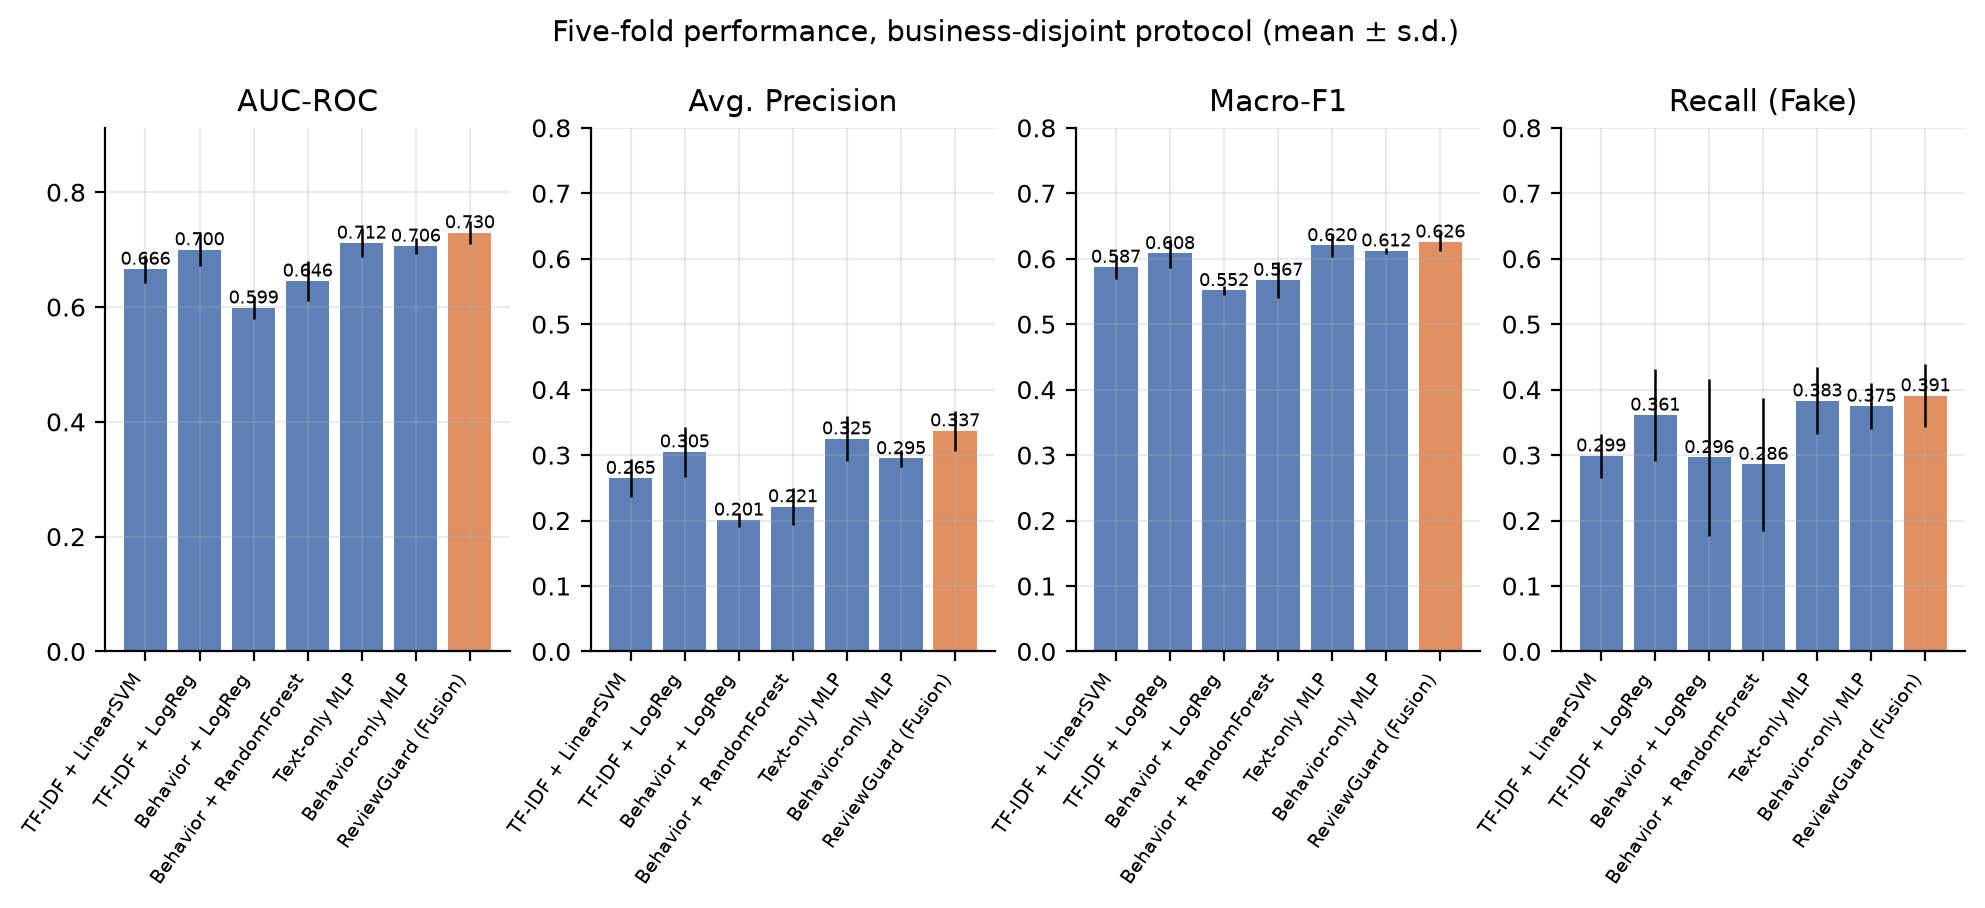
\includegraphics[width=\textwidth]{figures/final_model_comparison.png}
\caption{Five-fold performance under the business-disjoint protocol. Error bars
are standard deviations across folds.}
\label{fig:models}
\end{figure*}

ReviewGuard leads on every metric, at 0.730 AUC-ROC and 0.626 Macro-F1. These
are modest numbers, and we present them as the honest operating point for this
task rather than as a competitive result. Detecting a fake review at a business
one has never seen, from text and reviewer statistics alone and without usable
timestamps, is genuinely hard. The ordering of the two single branches is also
worth noting: text (0.712) slightly ahead of behavior (0.706), the reverse of
their ordering under the leakier protocol.

\subsection{Does Fusion Help?}

Table~\ref{tab:significance} tests ReviewGuard against each baseline.

% generated by src/make_tables.py -- do not edit
\begin{table}[htbp]
\caption{Wilcoxon signed-rank tests of ReviewGuard against each baseline over
the 5 folds of the business-disjoint protocol. $\Delta$ is the mean
per-fold advantage of ReviewGuard. $^{*}$ marks $p < 0.05$; with 5
paired folds the smallest attainable two-sided $p$-value is 0.0625, so no
comparison in this table can reach significance at $\alpha = 0.05$.}
\label{tab:significance}
\centering
\small
\begin{tabular}{llcc}
\toprule
\textbf{Baseline} & \textbf{Metric} & $\boldsymbol{\Delta}$ & \textbf{$p$} \\
\midrule
TF-IDF + LinearSVM & AUC-ROC & +0.064 & 0.062 \\
TF-IDF + LinearSVM & Macro-F1 & +0.038 & 0.062 \\
TF-IDF + LogReg & AUC-ROC & +0.030 & 0.062 \\
TF-IDF + LogReg & Macro-F1 & +0.018 & 0.062 \\
Behavior + LogReg & AUC-ROC & +0.131 & 0.062 \\
Behavior + LogReg & Macro-F1 & +0.074 & 0.062 \\
Behavior + RandomForest & AUC-ROC & +0.084 & 0.062 \\
Behavior + RandomForest & Macro-F1 & +0.058 & 0.062 \\
Text-only MLP & AUC-ROC & +0.018 & 0.062 \\
Text-only MLP & Macro-F1 & +0.006 & 0.125 \\
Behavior-only MLP & AUC-ROC & +0.023 & 0.125 \\
Behavior-only MLP & Macro-F1 & +0.014 & 0.125 \\
\bottomrule
\end{tabular}
\end{table}


Fusion improves on every baseline, and the improvement over the classical
models is large: $+0.084$ AUC over the behavioral random forest and $+0.131$
over behavioral logistic regression. Against its own ablations the margin is
smaller but consistent. ReviewGuard beats the text-only MLP on five of five
folds ($+0.018$ mean AUC) and the behavior-only MLP on four of five ($+0.024$).

We are deliberate about what this does and does not establish. With five paired
folds the Wilcoxon signed-rank test bottoms out at $p = 0.0625$, so the
five-of-five comparisons sit at the floor of what the test can report and
nothing here clears $\alpha = 0.05$. The effect is also small relative to
fold-to-fold spread, which Fig.~\ref{fig:stability} shows directly. We read the
evidence as a real but modest fusion benefit that, unlike the behavioral
advantage, survives the stricter protocol --- not as a decisive win. Whether a
transformer text branch would widen the margin is exactly the experiment we were
unable to run.

\begin{figure}[t]
\centering
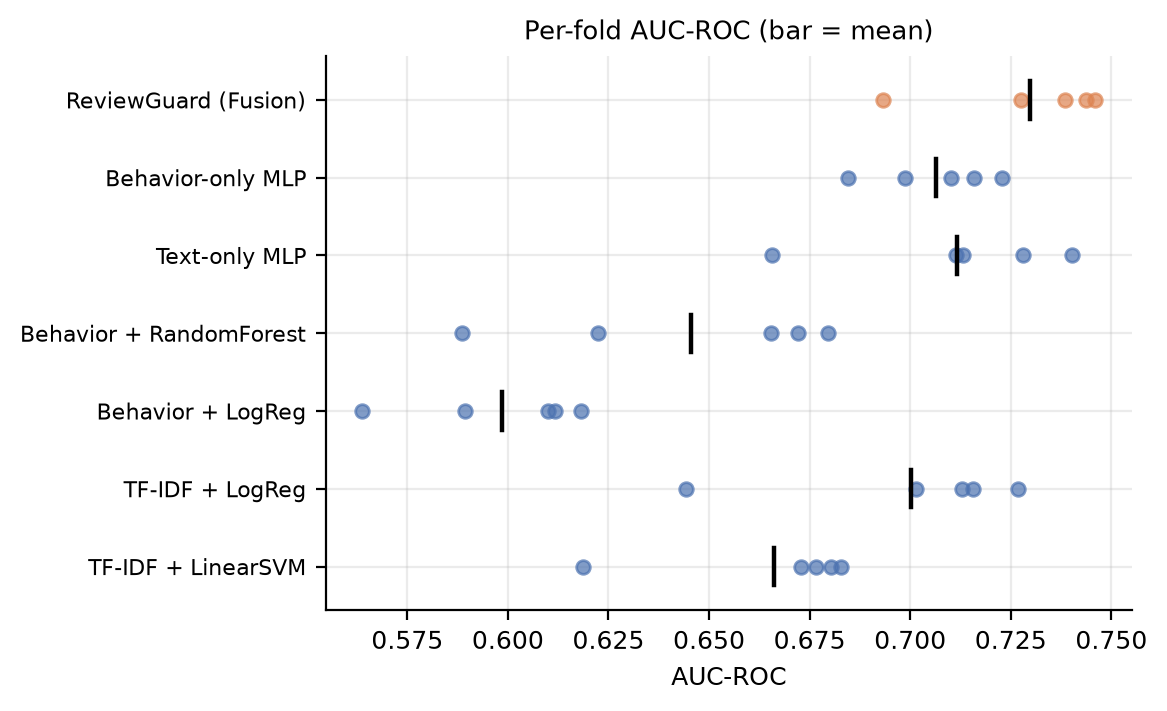
\includegraphics[width=\columnwidth]{figures/fold_stability.png}
\caption{Per-fold AUC-ROC under the business-disjoint protocol. Horizontal bars
mark per-model means. Fold-to-fold spread is comparable to the differences
between the leading models, which is why we decline to claim a fusion win.}
\label{fig:stability}
\end{figure}

\subsection{Discrimination and Errors}

Fig.~\ref{fig:roc} shows ROC curves and Fig.~\ref{fig:cm} the confusion matrix
for ReviewGuard. Both pool the out-of-fold predictions from all five
business-disjoint folds, so every review in the corpus is scored exactly once by
a model that never saw its business during training.

\begin{figure}[t]
\centering
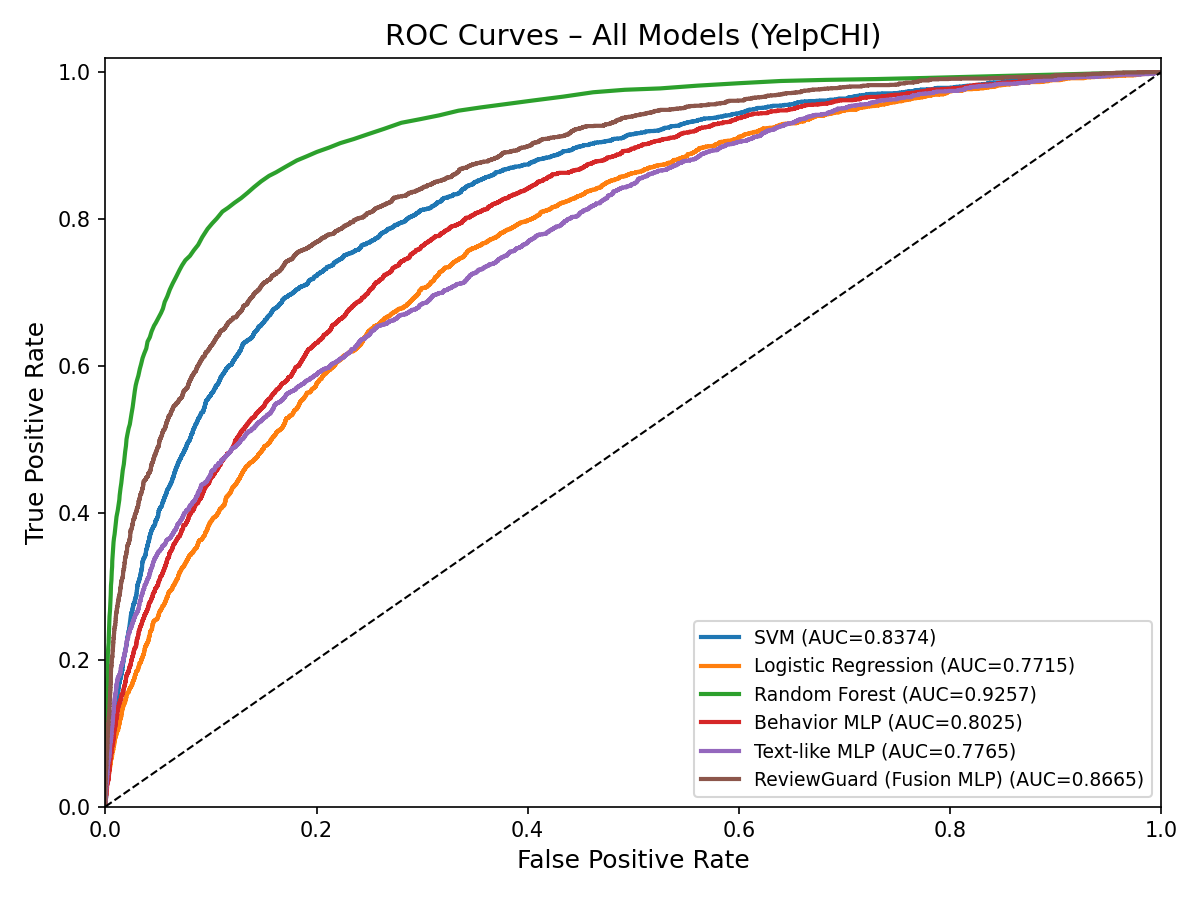
\includegraphics[width=\columnwidth]{figures/roc_all_models.png}
\caption{ROC curves for ReviewGuard and its two ablations, pooled over the
out-of-fold predictions of all five business-disjoint folds.}
\label{fig:roc}
\end{figure}

\begin{figure}[t]
\centering
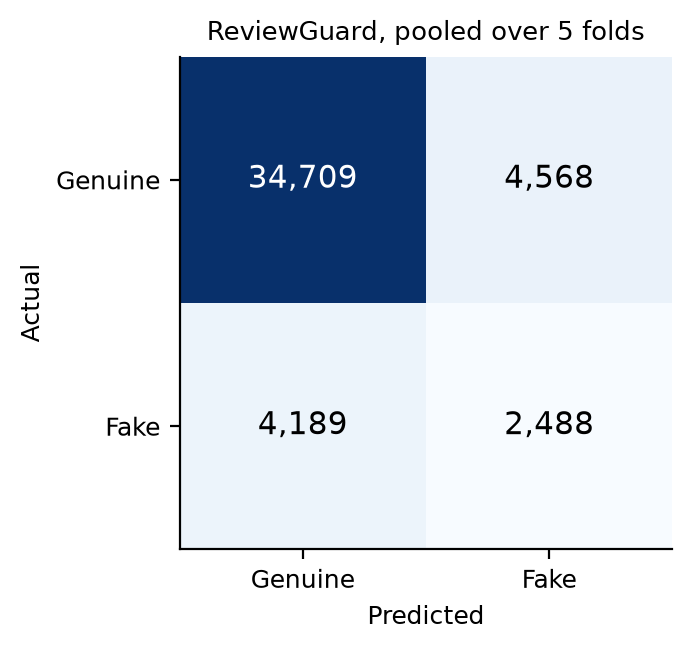
\includegraphics[width=0.82\columnwidth]{figures/cm_reviewguard_fusion.png}
\caption{ReviewGuard confusion matrix over the pooled out-of-fold predictions of
all five business-disjoint folds. A single threshold is fitted to the pooled
scores, giving 37.3\% fake-class recall against the 39.1\% mean of the
five per-fold thresholds in Table~\ref{tab:results}.}
\label{fig:cm}
\end{figure}

The error profile is what the threshold objective implies: tuning for Macro-F1
under 14.5\% prevalence buys fake-class recall at a substantial cost in false
positives. For deployment this trade-off should be set from the relative cost of
suppressing a genuine review versus missing a fake one, not from Macro-F1.

\subsection{What the Behavior Branch Actually Uses}

The protocol gap in Table~\ref{tab:protocol} shows that behavioral models rely
on business identity; SHAP~\cite{lundberg2017unified} attribution shows the
mechanism directly. Applying a kernel explainer to the behavior-only MLP over a
sample of held-out reviews, one feature dominates: \texttt{prod\_review\_count},
the number of reviews the business has received, carries a mean absolute SHAP
value of 0.462, five times that of the next feature
(\texttt{review\_word\_count}, 0.093). The four features describing the business
itself (\texttt{prod\_*}) account for 55.5\% of total attribution while making up
4 of the 19 inputs.

\begin{figure}[t]
\centering
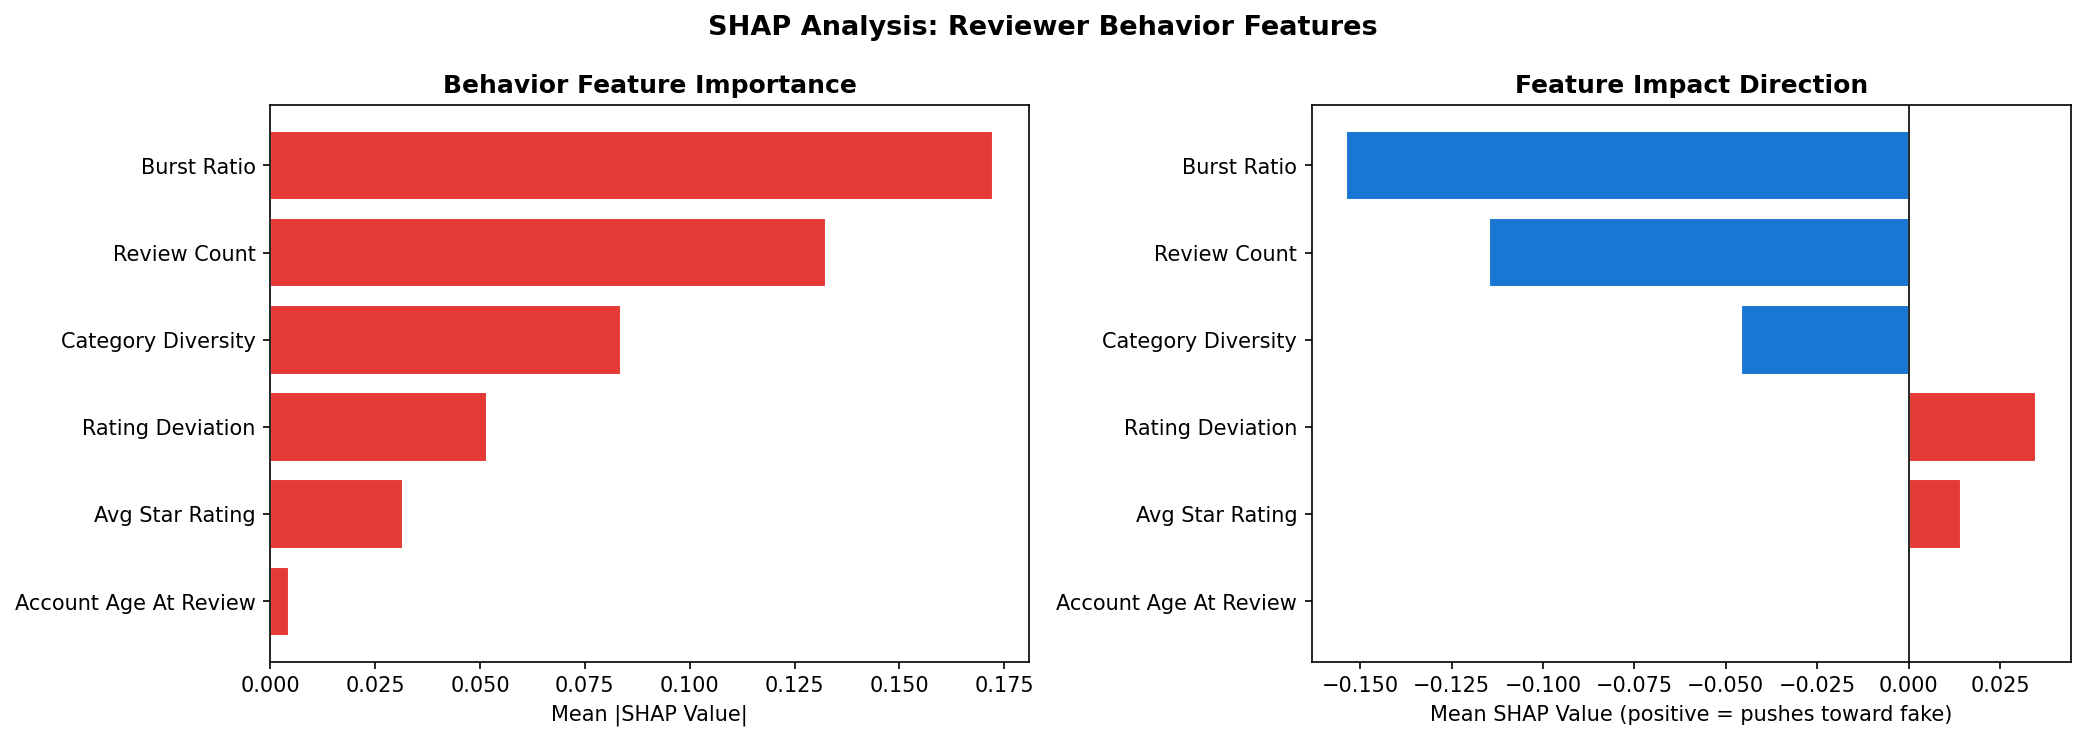
\includegraphics[width=\columnwidth]{figures/shap_behavior_summary.png}
\caption{Mean absolute SHAP value per behavioral feature for the behavior-only
MLP. Business-level features are shown in red. The single most influential
feature is how many reviews a business has received, which carries no
information about the review being classified.}
\label{fig:shap}
\end{figure}

This is worth stating plainly: the most influential input to the behavior branch
is a property of the business, not of the review or its author. Under the
reviewer-disjoint protocol that feature is highly predictive, because a business
seen in training carries its fake rate with it. Under the business-disjoint
protocol it is a bare popularity count for a business the model has never seen,
and its predictive value largely evaporates. The feature the model leans on
hardest is precisely the one that does not transfer.

% ============================================================
% VII. DISCUSSION
% ============================================================

\section{Discussion}
\label{sec:discussion}

\subsection{Implications for Benchmarking}

We do not claim that prior YelpCHI results are wrong. We claim that the standard
protocol does not separate two capabilities that behave very differently in
deployment: recognizing deception, and recognizing businesses with a history of
being targeted. Both are useful to a platform, and a platform monitoring a fixed
set of businesses may legitimately exploit the second. But a detector evaluated
only under a business-overlapping split has not been shown to do the first, and
its reported number will not survive contact with a new market. Reporting both
splits costs one extra run and makes the distinction visible.

The point generalizes past this dataset. Any fraud benchmark assembled by
sampling entities and collecting their records will concentrate labels by
entity, and any model given entity-level aggregates can exploit it.

\subsection{Limitations}

Our study has four limitations we consider material.

The text branch is lexical rather than transformer-based, for the
infrastructural reason given in Section~\ref{sec:method}. Our absolute numbers on
the text side should be read as a floor.

Timestamps are excluded because they are contaminated in the distribution
available to us, which removes the burstiness features that prior work found
valuable. A study using a clean temporal record would likely obtain a stronger
behavior branch, and should re-examine the protocol gap with those features
included --- burstiness is plausibly less business-specific than the aggregates
we use, and may transfer better.

Five folds admit no significance at $\alpha = 0.05$ under a signed-rank test,
whose smallest attainable two-sided $p$-value at $n = 5$ is 0.0625. Our
conclusions rest on effect sizes and fold-level consistency, and the fusion
comparison in particular is underpowered: a study wanting to settle it should
run repeated cross-validation or more folds.

Finally, YelpCHI's labels originate in Yelp's proprietary filter. They encode
one platform's operational definition of spam, with unknown false negative
rate, and both our results and the leakage we document are properties of that
labeling as much as of deception itself.

\subsection{Ethical Considerations}

At the operating points reported here, false positives substantially outnumber
true positives, and a false positive suppresses a genuine customer's review. A
system of this accuracy is appropriate for ranking a human moderation queue, not
for automated removal. We report Macro-F1 and per-class metrics rather than
accuracy specifically so that minority-class behavior stays visible.

% ============================================================
% VIII. CONCLUSION
% ============================================================

\section{Conclusion}
\label{sec:conclusion}

We set out to build a text-plus-behavior fake review detector for YelpCHI and
found that the benchmark's label structure makes conventional evaluation
misleading. Fake reviews cluster by business to the point that business identity
alone is a 0.951-AUC predictor, and models evaluated with businesses spanning the
split score far higher than the same models evaluated on unseen businesses. The
inflation is not uniform: it scales with how directly a model can reach business
identity, from 0.032 AUC for a text-only model to 0.289 for a behavioral random
forest, which is enough to reverse the ranking of behavioral and textual
features. We additionally document label-contaminated timestamps and an
uninformative behavioral feature file in a widely circulated distribution of the
dataset.

Under business-disjoint evaluation ReviewGuard reaches 0.730 AUC-ROC, ahead of
both of its ablations, though by a margin that five folds cannot establish as
significant. We think those numbers, and not the higher ones obtainable under a
weaker protocol, are the ones worth reporting.

Three directions follow. First, completing the transformer text branch, which
our infrastructure prevented and which is the most likely source of improvement.
Second, re-examining published YelpCHI and YelpNYC results under
business-disjoint splits, particularly for graph-based methods, which have the
most direct access to business identity. Third, obtaining a clean temporal
record so that burstiness features can be evaluated for whether they transfer
across businesses as poorly as static aggregates do.

\section*{Acknowledgment}

The authors thank Prof.\ Song Fang of the School of Computer Science,
University of Oklahoma, for guidance throughout this project.

\section*{Reproducibility}

Code, the data integrity audit, and the metrics behind every table and figure in
this paper are available in the project repository. All result tables are
generated programmatically from the recorded metrics files rather than
transcribed by hand.

% ============================================================
% REFERENCES
% ============================================================

\bibliographystyle{IEEEtran}

\begin{thebibliography}{20}

\bibitem{luca2016fake}
M.~Luca and G.~Zervas, ``Fake it till you make it: Reputation, competition, and Yelp review fraud,'' \textit{Management Science}, vol.~62, no.~12, pp.~3412--3427, 2016.

\bibitem{crothers2023machine}
E.~Crothers, N.~Japkowicz, and H.~Viktor, ``Machine-generated text: A comprehensive survey of threat models and detection methods,'' \textit{IEEE Access}, vol.~11, pp.~70977--71002, 2023.

\bibitem{rayana2015collective}
S.~Rayana and L.~Akoglu, ``Collective opinion spam detection: Bridging review networks and metadata,'' in \textit{Proc. ACM KDD}, Sydney, Australia, 2015, pp.~985--994.

\bibitem{ott2011finding}
M.~Ott, Y.~Choi, C.~Cardie, and J.~T.~Hancock, ``Finding deceptive opinion spam by any stretch of the imagination,'' in \textit{Proc. ACL}, Portland, OR, 2011, pp.~309--319.

\bibitem{jindal2008opinion}
N.~Jindal and B.~Liu, ``Opinion spam and analysis,'' in \textit{Proc. ACM WSDM}, Palo Alto, CA, 2008, pp.~219--230.

\bibitem{mukherjee2013what}
A.~Mukherjee, V.~Venkataraman, B.~Liu, and N.~S.~Glance, ``What Yelp fake review filter might be doing?,'' in \textit{Proc. ICWSM}, Cambridge, MA, 2013, pp.~409--418.

\bibitem{devlin2019bert}
J.~Devlin, M.-W.~Chang, K.~Lee, and K.~Toutanova, ``BERT: Pre-training of deep bidirectional transformers for language understanding,'' in \textit{Proc. NAACL-HLT}, Minneapolis, MN, 2019, pp.~4171--4186.

\bibitem{liu2019roberta}
Y.~Liu, M.~Ott, N.~Goyal, J.~Du, M.~Joshi, D.~Chen, O.~Levy, M.~Lewis, L.~Zettlemoyer, and V.~Stoyanov, ``RoBERTa: A robustly optimized BERT pretraining approach,'' arXiv:1907.11692, 2019.

\bibitem{kipf2017semi}
T.~N.~Kipf and M.~Welling, ``Semi-supervised classification with graph convolutional networks,'' in \textit{Proc. ICLR}, Toulon, France, 2017.

\bibitem{wang2020attributed}
Z.~Wang, K.~Hou, D.~Song, Z.~Li, T.~Zhang, and G.~Hu, ``Attributed graph neural network for fake review detection,'' in \textit{Proc. IEEE ICDM}, Sorrento, Italy, 2020, pp.~621--630.

\bibitem{kaufman2012leakage}
S.~Kaufman, S.~Rosset, C.~Perlich, and O.~Stitelman, ``Leakage in data mining: Formulation, detection, and avoidance,'' \textit{ACM Trans. Knowledge Discovery from Data}, vol.~6, no.~4, pp.~1--21, 2012.

\bibitem{geirhos2020shortcut}
R.~Geirhos, J.-H.~Jacobsen, C.~Michaelis, R.~Zemel, W.~Brendel, M.~Bethge, and F.~A.~Wichmann, ``Shortcut learning in deep neural networks,'' \textit{Nature Machine Intelligence}, vol.~2, no.~11, pp.~665--673, 2020.

\bibitem{lin2017focal}
T.-Y.~Lin, P.~Goyal, R.~Girshick, K.~He, and P.~Doll\'{a}r, ``Focal loss for dense object detection,'' in \textit{Proc. IEEE ICCV}, Venice, Italy, 2017, pp.~2980--2988.

\bibitem{kingma2015adam}
D.~P.~Kingma and J.~Ba, ``Adam: A method for stochastic optimization,'' in \textit{Proc. ICLR}, San Diego, CA, 2015.

\bibitem{cortes1995support}
C.~Cortes and V.~Vapnik, ``Support-vector networks,'' \textit{Machine Learning}, vol.~20, no.~3, pp.~273--297, 1995.

\bibitem{lundberg2017unified}
S.~M.~Lundberg and S.-I.~Lee, ``A unified approach to interpreting model predictions,'' in \textit{Proc. NeurIPS}, Long Beach, CA, 2017, pp.~4765--4774.

\bibitem{breiman2001random}
L.~Breiman, ``Random forests,'' \textit{Machine Learning}, vol.~45, no.~1, pp.~5--32, 2001.

\end{thebibliography}

\balance

\end{document}
